\documentclass[11pt]{article}

% Page layout
\usepackage[margin=1in]{geometry}

% Math
\usepackage{amsmath}
\usepackage{amssymb}

% Tables
\usepackage{booktabs}
\usepackage{multirow}
\usepackage{array}

% Graphics and figures
\usepackage{graphicx}
\usepackage{tikz}
\usetikzlibrary{positioning, arrows.meta, calc}

% Colors
\usepackage{xcolor}

% Lists
\usepackage{enumitem}

% Float control
\usepackage{float}

% Code listings
\usepackage{listings}
\lstset{
  basicstyle=\ttfamily\small,
  breaklines=true,
  frame=single,
  columns=fullflexible
}

% Hyperlinks
\usepackage{hyperref}
\hypersetup{
  colorlinks=true,
  linkcolor=blue!60!black,
  citecolor=blue!60!black,
  urlcolor=blue!60!black
}

% Citations
\usepackage{natbib}
\bibliographystyle{plainnat}

% Title
\title{Ploidy: Context-Asymmetric Structured Debate\\for LLM Decision Verification}
\author{heznpc}
\date{}

\begin{document}

\maketitle

% ============================================================
% Abstract
% ============================================================
\begin{abstract}
Single-session LLM usage subjects critical decisions to stochastic prior lock-in: the model's first probabilistic response anchors all subsequent reasoning, and prompt-based mitigations have no statistically significant effect on this bias~\citep{feng2026anchoring}. We present Ploidy, a structured debate protocol between physically separate sessions of the same model with intentionally asymmetric context depths. Unlike multi-model council approaches that rely on model diversity, Ploidy exploits \textbf{context diversity} within a single model---a dimension absent from existing products and publications as of March 2026. We introduce the \textbf{Context Asymmetry Spectrum}, which varies along two dimensions: context depth (how much prior knowledge a session receives) and context delivery mode (whether context is passively embedded or actively retrievable). Sessions range from Deep (full context, always present) through Semi-Fresh (compressed context, passively or actively delivered) to Fresh (zero context), debating through typed semantic actions before a convergence phase. In preliminary pilot experiments on 10 tasks across two context regimes, we observe that (1)~context asymmetry provides no benefit on short-context tasks where entrenchment does not occur, and (2)~on long-context tasks with anchoring bias, asymmetric debate achieves the highest ground-truth recall on the most bias-laden task (5/5 vs.\ Single Session's 3/5, stable across re-runs). These results bound where context asymmetry applies. In a follow-up evaluation of Semi-Fresh variants with factorial ablation, we identify \textbf{information position as the dominant factor}: placing a compressed summary at the end rather than the beginning of the prompt improves recall from 89\% to 100\%, consistent with primacy anchoring effects in human cognition. We release Ploidy as an open-source MCP server.
\end{abstract}

% ============================================================
\section{Introduction}
\label{sec:introduction}
% ============================================================

LLM outputs are stochastic. The same model, given the same prompt, produces different responses across independent sessions. This is well-understood. What is less appreciated is the downstream consequence for single-session workflows:

\begin{enumerate}[label=\arabic*.]
  \item The model's first response is sampled from a probability distribution.
  \item That response enters the context window and becomes the model's own prior.
  \item The model reinforces this prior through consistency-seeking behavior (anchoring bias, sycophancy).
  \item The user sees only one session and treats the output as deterministic.
\end{enumerate}

The result: identical models, identical prompts, identical users---but different project outcomes depending on which stochastic sample landed first. Jacob et al.~\citep{jacob2025chatchamber} term this the ``Chat-Chamber Effect''---the tendency for users to trust and build upon whatever stochastic output a single session produces. This is not addressable by temperature tuning or prompt engineering; empirical evidence shows prompt-based mitigations (chain-of-thought, reflection, ``ignore your prior response'') have no statistically significant effect on anchoring bias~\citep{feng2026anchoring}.

This phenomenon has a well-documented human analog: accumulated expertise simultaneously enables domain mastery and prevents paradigm revision---a dynamic observed across scientific communities~\citep{kuhn1962structure}, empirically confirmed in studies of eminent scientists' influence on field renewal~\citep{azoulay2019funeral}, and formalized as a structural property of generational turnover. We explore this parallel in depth in a companion paper; here, we note only that the LLM single-session problem is structurally similar---context accumulation creates anchoring that prompt-based interventions cannot overcome~\citep{feng2026anchoring}.

The practical consequence is stark: given the same model and the same prompt, different sessions may produce fundamentally different assessments---agree, disagree, or equivocate---on the same hypothesis. A user confined to a single session is unknowingly subject to a stochastic lottery whose outcome determines not just the quality of individual responses, but whether entire tasks succeed or fail. Two users with identical models and identical problems may experience dramatically different ``model performance'' based solely on which stochastic sample anchored their session.

The only computational intervention with empirical support for this problem is physical session separation. Cross-Context Review (CCR)~\citep{song2026ccr} demonstrated that a fresh session reviewing an artifact produced by a deep session achieves F1=28.6\% on error detection versus 24.6\% for same-session review ($p=0.008$). However, CCR is unidirectional---the fresh session reviews but does not debate.

We extend CCR from unidirectional review to \textbf{bidirectional structured debate} and introduce the \textbf{Context Asymmetry Spectrum}---a continuum from full context (Deep) through compressed context (Semi-Fresh) to zero context (Fresh). This spectrum recognizes that the optimal information state for a challenger may be neither complete ignorance nor full knowledge, but an intermediate point analogous to the ``experienced outsider'' who brings domain awareness without institutional entrenchment.

\paragraph{Contributions.}
\begin{itemize}[leftmargin=1.5em]
  \item The Context Asymmetry Spectrum: a framework for reasoning about optimal context depth in multi-session verification (\S\ref{sec:protocol})
  \item A structured debate protocol with typed semantic actions and convergence analysis (\S\ref{sec:protocol})
  \item Preliminary pilot experiments (10 tasks, two context regimes) with honest null and qualified positive results (\S\ref{sec:experiments})
  \item Analysis of when context asymmetry helps and when it does not, bounding the intervention's applicability (\S\ref{sec:discussion})
  \item An open-source MCP server implementation (\S\ref{sec:implementation})
\end{itemize}

% ============================================================
\section{Background and Related Work}
\label{sec:related}
% ============================================================

\subsection{Context Degradation in Long Sessions}
\label{sec:context-degradation}

LLM performance degrades with context length even when retrieval is perfect---Du et al.~\citep{du2025context} showed 13.9--85\% performance drops that are architectural, not retrieval-related. Chroma Research~\citep{chroma2025contextrot} evaluated 18 frontier models and found effective context capacity is approximately 60--70\% of advertised window size. The ``scaling paradox''~\citep{scaling2026paradox} further shows that larger context compressors produce less faithful reconstructions due to knowledge overwriting.

\subsection{Multi-Agent Debate}
\label{sec:mad}

Multi-agent debate (MAD) is well-studied but predominantly uses symmetric configurations where all agents share the same context. Recent work has explored multi-LLM context learning for richer discussion dynamics~\citep{m2cl2026}, but the fundamental assumption of shared context remains. Oh et al.~\citep{oh2025dreamad} demonstrated that symmetric debate can amplify bias through ``belief entrenchment.'' Choi et al.~\citep{choi2025debate} proved that debate under symmetric information induces a martingale---it cannot improve expected correctness beyond majority voting. This result has implications beyond LLMs: any system where agents share identical priors and debate cannot, in expectation, improve upon aggregating their independent judgments.

\subsection{Asymmetric Context as a Mechanism}
\label{sec:asymmetric}

SR-DCR~\citep{srdcr2025} introduced asymmetric context verification debate (ACVD): a context-defending agent debates a context-deprived critic. On GPT-3.5, this achieved 62.7\% accuracy (+3.4pp over naive debate). AceMAD~\citep{liu2026acemad} proved that asymmetric cognitive potential creates submartingale drift toward truth, formally breaking the martingale curse. We note that Ploidy's current single-round design does not satisfy the multi-round conditions required for AceMAD's submartingale proof; whether a multi-round extension would achieve this remains an open question (\S\ref{sec:conclusion}).

\subsection{Scaling Agents vs.\ Scaling Diversity}
\label{sec:scaling}

Large-scale agent simulations (e.g., AgentSociety~\citep{pang2025agentsociety} with 10K agents, MiroFish with 700K agents) pursue verification breadth---more agents analyzing the same problem. Boca et al.~\citep{boca2025emergent} showed that even without individual-level bias, LLM populations spontaneously develop collective biases through interaction. Combined with Choi et al.'s martingale result~\citep{choi2025debate}, this suggests that scaling homogeneous agent count does not reliably improve decision quality. Ploidy pursues the orthogonal dimension: verification depth through context diversity.

\subsection{Model Collapse and Context Contamination}
\label{sec:collapse}

When AI-generated content enters training data, progressive quality degradation occurs---``model collapse''~\citep{shumailov2024collapse}. Ploidy's design of maintaining sessions with different context depths is a within-deployment countermeasure to this homogenization tendency.

\subsection{Ploidy's Position}
\label{sec:position}

\begin{table}[t]
\centering
\caption{Comparison of Ploidy with prior work along key design dimensions.}
\label{tab:prior-work}
\footnotesize
\setlength{\tabcolsep}{4pt}
\begin{tabular}{@{}p{3.2cm}p{2.4cm}p{3cm}p{2.2cm}p{3cm}@{}}
\toprule
\textbf{Prior Work} & \textbf{Mechanism} & \textbf{Context Depth} & \textbf{Delivery} & \textbf{Direction} \\
\midrule
CCR~\citep{song2026ccr} & Session separation & Binary (Deep/Fresh) & Passive & Unidirectional review \\[3pt]
SR-DCR/ACVD~\citep{srdcr2025} & Asymmetric debate & Binary (Defender/Critic) & Passive & Unidirectional + Judge \\[3pt]
AceMAD~\citep{liu2026acemad} & Asymmetric potential & Theoretical & n/a & Multi-round proof \\[3pt]
AgentSociety~\citep{pang2025agentsociety} & Population simulation & Homogeneous & Passive & Observation only \\[3pt]
\textbf{Ploidy} & \textbf{Structured debate} & \textbf{Spectrum (Deep$\to$Fresh)} & \textbf{Passive + Active} & \textbf{Bidirectional + convergence} \\
\bottomrule
\end{tabular}
\end{table}

\subsection{Distinction from Multi-Agent Task Division}
\label{sec:distinction}

Claude Agent Teams and similar systems (CrewAI, MetaGPT) implement cooperative division---splitting work across agents for throughput. Adding more agents increases throughput (more hands) but does not address anchoring bias, because all agents share the same context and thus the same stochastic priors. Under Choi et al.'s martingale result~\citep{choi2025debate}, scaling homogeneous agents is mathematically equivalent to majority voting over identically biased samples. Ploidy implements the orthogonal strategy: cooperative verification, where the same problem is analyzed from intentionally different information states. The goal is not more output but different perspectives---disagreements are the primary signal, not a failure mode.

% ============================================================
\section{The Ploidy Protocol}
\label{sec:protocol}
% ============================================================

\subsection{The Context Asymmetry Spectrum}
\label{sec:spectrum}

Prior work treats context as binary: full context vs.\ no context. We propose a two-dimensional spectrum defined by \textbf{context depth} and \textbf{context delivery mode}.

\textbf{Context depth} determines how much prior knowledge a session receives:

\begin{figure}[t]
\centering
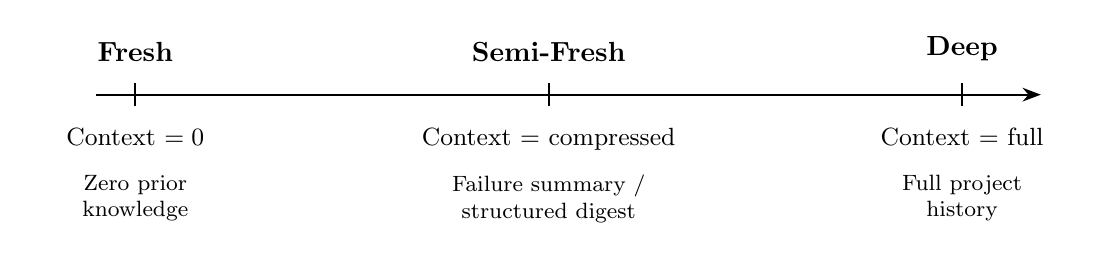
\begin{tikzpicture}[>=Stealth, node distance=0.5cm]
  % Main axis line
  \draw[thick, ->] (0,0) -- (12,0);

  % Tick marks and labels
  \draw[thick] (0.5,-0.15) -- (0.5,0.15);
  \draw[thick] (5.75,-0.15) -- (5.75,0.15);
  \draw[thick] (11,-0.15) -- (11,0.15);

  % Top labels (session names)
  \node[above, font=\bfseries] at (0.5, 0.3) {Fresh};
  \node[above, font=\bfseries] at (5.75, 0.3) {Semi-Fresh};
  \node[above, font=\bfseries] at (11, 0.3) {Deep};

  % Context values
  \node[below, font=\small] at (0.5, -0.3) {Context $= 0$};
  \node[below, font=\small] at (5.75, -0.3) {Context $=$ compressed};
  \node[below, font=\small] at (11, -0.3) {Context $=$ full};

  % Descriptions below
  \node[below, font=\footnotesize, text width=2.5cm, align=center] at (0.5, -0.9) {Zero prior\\knowledge};
  \node[below, font=\footnotesize, text width=3cm, align=center] at (5.75, -0.9) {Failure summary /\\structured digest};
  \node[below, font=\footnotesize, text width=2.5cm, align=center] at (11, -0.9) {Full project\\history};
\end{tikzpicture}
\caption{The Context Depth Spectrum: sessions range from zero prior knowledge (Fresh) through compressed summaries (Semi-Fresh) to full project history (Deep).}
\label{fig:spectrum}
\end{figure}

\begin{itemize}[leftmargin=1.5em]
  \item \textbf{Deep}: Full project context---codebase, decision history, accumulated knowledge. Maximizes domain awareness but risks anchoring bias.
  \item \textbf{Semi-Fresh}: Compressed context---a structured summary of prior attempts, known constraints, or failure modes, without the full narrative that induces entrenchment. Analogous to an experienced outsider or a practitioner restarting a stuck project with lessons learned but freed from sunk-cost attachment.
  \item \textbf{Fresh}: Zero prior context---only the raw artifact under review. Maximizes independence but lacks domain constraints.
\end{itemize}

\textbf{Context delivery mode} determines how context reaches the session, independently of depth:

\begin{itemize}[leftmargin=1.5em]
  \item \textbf{Passive delivery}: Context is embedded directly in the prompt and is always present in the context window. Every response is implicitly influenced by this context, whether or not it is relevant to the specific question being answered. This mirrors the expert whose 20 years of experience unconsciously shapes every judgment.
  \item \textbf{Active delivery}: Context is available through an explicit retrieval mechanism (e.g., a tool call) but is not present in the window until requested. The session must decide when and whether to consult prior knowledge. This mirrors the consultant who researches on demand rather than relying on ingrained assumptions.
\end{itemize}

The same information, delivered passively vs.\ actively, may produce different entrenchment dynamics. This prediction is grounded in established cognitive science findings: the generation effect~\citep{slamecka1978generation} shows that actively produced knowledge is more deeply processed than passively received information, and the testing effect~\citep{roediger2006test} demonstrates that retrieval practice outperforms re-reading for durable learning. Passive delivery maximizes the risk of anchoring bias (the context is always ``priming'' the model), while active delivery introduces a selection step that may reduce entrenchment---the session must formulate a query, which requires some metacognitive awareness of what it does not know. Epley and Gilovich~\citep{epley2006anchoring} showed that anchoring operates through different mechanisms for externally provided vs.\ self-generated anchors, further supporting the prediction that delivery mode matters independently of content.

\begin{figure}[t]
\centering
\caption{The Context Asymmetry Spectrum: a 2D space defined by context depth (rows) and delivery mode (columns), yielding five distinct session configurations.}
\label{fig:2d-matrix}
\vspace{0.5em}
\small
\begin{tabular}{@{} >{\bfseries}l c c c @{}}
\toprule
& \textbf{Passive} & \textbf{Active} & \textbf{None} \\
& \footnotesize(always in window) & \footnotesize(tool/retrieval) & \footnotesize(absent) \\
\midrule
Full
  & Deep & Deep-Active & \multirow{1}{*}{\textcolor{gray}{n/a}} \\
  & \footnotesize\textit{(expert intuition)} & \footnotesize\textit{(expert + lookup)} & \\[6pt]
Compressed
  & Semi-Fresh-Passive & Semi-Fresh-Active & \multirow{1}{*}{\textcolor{gray}{n/a}} \\
  & \footnotesize\textit{(briefed outsider)} & \footnotesize\textit{(consultant)} & \\[6pt]
None
  & \textcolor{gray}{n/a} & \textcolor{gray}{n/a} & Fresh \\
  & & & \footnotesize\textit{(novice)} \\
\bottomrule
\end{tabular}
\end{figure}

This 2D space yields five distinct session configurations. The current implementation supports Deep (full/passive) and Fresh (none). Semi-Fresh variants and Active delivery are proposed as key extensions (\S\ref{sec:semifresh}, \S\ref{sec:conclusion}).

\subsection{Architecture}
\label{sec:architecture}

MCP client sessions connect to a single Ploidy server via Streamable HTTP:

\begin{itemize}[leftmargin=1.5em]
  \item \textbf{Deep session}: Full project context (codebase, history, prior decisions)
  \item \textbf{Fresh session}: Only the raw artifact under review (code snippet, architecture question)
  \item \textbf{Semi-Fresh session} (proposed): Deep's \textsc{position} output, compressed by a summarization step, as the only context
\end{itemize}

The server maintains debate state in SQLite (WAL mode) and enforces the phase protocol.

\subsection{Debate Phases}
\label{sec:phases}

\begin{enumerate}[label=\arabic*., leftmargin=1.5em]
  \item \textbf{Position}: All sessions independently analyze the artifact. Each produces a list of findings with confidence levels.
  \item \textbf{Challenge}: Each session reviews the others' positions. For each finding, the reviewer responds with a typed semantic action:
  \begin{itemize}[leftmargin=1em]
    \item \texttt{agree}---finding is valid
    \item \texttt{challenge}---finding is wrong or misleading, with explanation
    \item \texttt{propose\_alternative}---finding is partially right, here's a different framing
    \item \texttt{synthesize}---combining both perspectives into a stronger finding
  \end{itemize}
  \item \textbf{Convergence}: The protocol analyzes the debate transcript and classifies outcomes:
  \begin{itemize}[leftmargin=1em]
    \item \textbf{Agreements}: findings confirmed by multiple sessions
    \item \textbf{Productive disagreements}: findings where challenge/synthesis produced new insight
    \item \textbf{Irreducible disagreements}: genuine differences that could not be resolved
    \item \textbf{Confidence score}: proportion of agreed findings
  \end{itemize}
\end{enumerate}

\subsection{Design Principles}
\label{sec:principles}

\begin{itemize}[leftmargin=1.5em]
  \item \textbf{No shared memory}: Fresh/Semi-Fresh sessions never see Deep's raw analysis outside the debate protocol.
  \item \textbf{Typed actions over free-form}: Semantic actions make the debate transcript machine-interpretable.
  \item \textbf{Disagreement as signal}: Irreducible disagreements are informative, not failures---they mark where context mattered.
\end{itemize}

% ============================================================
\section{Implementation}
\label{sec:implementation}
% ============================================================

Ploidy is implemented as a Python MCP server (FastMCP, asyncio, aiosqlite) exposing 10 tools over Streamable HTTP on port 8765. The server manages debate lifecycle, enforces phase transitions via a finite state machine (\textsc{independent} $\to$ \textsc{position} $\to$ \textsc{challenge} $\to$ \textsc{convergence} $\to$ \textsc{complete}), and persists all state in SQLite with WAL mode for crash recovery. Per-debate asyncio locks guard concurrent phase transitions.

\paragraph{v0.2 enhancements.} The implementation now includes:
\begin{itemize}[leftmargin=1.5em]
  \item \textbf{Semi-Fresh sessions}: Native server support for sessions with compressed context, delivered passively (in-prompt) or actively (retrieval-after-independent-analysis).
  \item \textbf{API fallback} (\texttt{debate\_auto}): Single-command debate via OpenAI-compatible API endpoints. The server auto-generates Fresh or Semi-Fresh responses, enabling single-terminal workflows. Supports any backend (Anthropic, OpenAI, Ollama, OpenRouter).
  \item \textbf{LLM-enhanced convergence}: Optional meta-analysis that uses an LLM to explain \emph{why} sessions disagreed, attributing disagreements to specific context factors (sunk cost bias, missing domain constraints, stochastic variance, or genuine trade-offs).
  \item \textbf{Visualization dashboard}: Read-only web interface for browsing debate history, timelines, and convergence results from the SQLite database.
  \item \textbf{Effort level}: Configurable reasoning depth parameter that controls how much computation the model applies per response---an experimental variable that may interact with context asymmetry (\S\ref{sec:effort}).
\end{itemize}

We note that the experiments in \S\ref{sec:experiments} use the \texttt{claude --print} CLI to simulate the protocol rather than the MCP server directly, as this provides cleaner session isolation for controlled comparison. Each CLI invocation creates a guaranteed-fresh session with no shared state. The MCP server is designed for production use where two human-operated terminals connect to the same server instance.

Full source: \url{https://github.com/heznpc/ploidy}

% ============================================================
\section{Experiments}
\label{sec:experiments}
% ============================================================

This section reports preliminary pilot results. All findings should be interpreted as observations from a small-scale pilot study, not as statistically validated conclusions. We report both null and positive observations to bound where context asymmetry applies.

\subsection{Setup}
\label{sec:setup}

We evaluate on 10 tasks across two context regimes:
\begin{itemize}[leftmargin=1.5em]
  \item \textbf{Experiment~1} (short context, $\sim$50 tokens): 5 code review tasks with injected bugs + 2 architecture decision tasks. Each has 3--5 ground-truth issues.
  \item \textbf{Experiment~2} (long context, 2,000--5,000 tokens): 3 architecture decision tasks with project histories containing anchoring-inducing biases. Each has 5--6 ground-truth issues.
\end{itemize}

\paragraph{Methods} (all using Claude Opus 4.6 via \texttt{claude --print}, each invocation = fresh session):
\begin{enumerate}[label=\arabic*., leftmargin=1.5em]
  \item \textbf{Single Session}: One session with full context.
  \item \textbf{Independent Second Opinion}: Two sessions with full context, responses concatenated.
  \item \textbf{CCR (Unidirectional)}: Deep session produces analysis; Fresh session reviews it.
  \item \textbf{Symmetric Debate}: Two sessions with identical full context debate each other.
  \item \textbf{Ploidy (Asymmetric Debate)}: Deep (full context) vs Fresh (zero context), structured protocol.
  \item \textbf{Self-Consistency (5-vote)}: Five independent single sessions, majority-vote synthesis. Approximately equal token budget to Ploidy ($\sim$5 LLM calls).
  \item \textbf{Semi-Fresh-Passive}: Deep session produces analysis; compressed summary injected directly into Semi-Fresh session's prompt.
  \item \textbf{Semi-Fresh-Active}: Deep session produces analysis; compressed summary available to Semi-Fresh session but only after independent assessment. Session must form its own view first, then consult prior analysis.
  \item \textbf{Semi-Fresh-Selective}: Deep session produces analysis; only failure/uncertainty information extracted and provided to Semi-Fresh session.
\end{enumerate}

\paragraph{Judge.} Claude Opus 4.6 evaluates each method's output against ground truth. For each ground-truth issue: \textsc{found}~(1.0), \textsc{partial}~(0.5), or \textsc{missed}~(0.0). Additional valid findings not in ground truth are counted separately as bonus findings.

\paragraph{Metrics.} Recall $= (\text{found} + 0.5 \times \text{partial}) / \text{total ground truth}$. Precision and F1 are reported but include bonus findings in the denominator, which penalizes methods that produce more valid-but-unlisted findings. We flag this as a metric design issue (\S\ref{sec:why-no-help}) and recommend interpreting recall as the primary indicator of ground-truth detection.

\paragraph{Effort level.} Claude Code exposes an \textbf{effort} parameter (low, medium, high, max) that controls the model's reasoning depth per response. All experiments in this paper use the default \texttt{high} effort unless otherwise noted. We identify effort level as a potentially confounding variable: lower effort may reduce a session's ability to detect subtle issues, while higher effort may increase the quality of challenges. In \S\ref{sec:effort}, we describe a factorial experiment design crossing effort levels with methods to measure this interaction.

\paragraph{Limitations of this setup} (expanded in \S\ref{sec:limitations}): single run per method-task pair, author-defined ground truth without independent validation, same model family as judge, CLI simulation rather than MCP server execution, and single effort level.

\subsection{Results (Experiment 1: Short-Context Tasks)}
\label{sec:exp1-results}

7 tasks (5 code review + 2 architecture), Claude Opus 4.6, single run per method.

\begin{table}[t]
\centering
\caption{Experiment~1 results: short-context tasks ($\sim$50 tokens). All 9 methods achieve near-perfect recall.}
\label{tab:exp1}
\small
\begin{tabular}{@{}lccc@{}}
\toprule
\textbf{Method} & \textbf{Avg F1} & \textbf{Avg Recall} & \textbf{Avg Time} \\
\midrule
Single Session            & \textbf{0.573} & 3.7/4.1 & 40s  \\
Second Opinion            & 0.554          & 4.1/4.1 & 89s  \\
Symmetric Debate          & 0.555          & 4.0/4.1 & 118s \\
CCR (Unidirectional)      & 0.548          & 3.9/4.1 & 92s  \\
Ploidy (Asymmetric)       & 0.540          & 3.9/4.1 & 205s \\
Semi-Fresh-Active         & 0.538          & 3.9/4.1 & 117s \\
Semi-Fresh-Passive        & 0.535          & 3.9/4.1 & 122s \\
Semi-Fresh-Selective      & 0.533          & 4.0/4.1 & 130s \\
Self-Consistency (5-vote) & 0.529          & 3.7/4.1 & 234s \\
\bottomrule
\end{tabular}
\end{table}

\textbf{Observation: No method consistently outperforms Single Session on these tasks.} All 9 methods achieve near-perfect recall (90--98\%), and F1 differences are driven by precision (bonus findings inflating denominators). Critically, the delivery mode effect observed in Experiment~2 (SF-Active vs SF-Passive) disappears entirely here: both achieve identical 3.9/4.1 recall. This confirms that context asymmetry and delivery mode provide no benefit when context is too short for entrenchment to occur.

\subsection{Analysis: Why Context Asymmetry Did Not Help}
\label{sec:why-no-help}

\textbf{1.\ Insufficient context depth.} Each task's project context was $\sim$50 tokens. Context entrenchment requires accumulated context on the order of thousands of tokens. At 50 tokens, the Deep session develops no meaningful anchoring bias.

\textbf{2.\ Task difficulty ceiling.} Claude Opus 4.6 found nearly all ground-truth issues in every method. When baseline recall is near-perfect, multi-session methods cannot demonstrate improvement.

\textbf{3.\ Metric design issue.} Our F1 formulation includes bonus findings (valid issues not in ground truth) in the precision denominator. This systematically penalizes more thorough methods. A revised metric should either exclude bonus findings from precision or report them as a separate axis. We retain the current formulation for transparency but caution against interpreting F1 differences smaller than the observed stochastic variance ($\pm 0.10$).

\subsection{Qualitative Observations}
\label{sec:qualitative}

Despite quantitative parity, Ploidy's convergence phase produced qualitatively distinct outputs:

\begin{itemize}[leftmargin=1.5em]
  \item \textbf{Severity calibration}: Fresh session challenged Deep's severity escalation of a memory leak, arguing it depends on key cardinality---a nuance absent from single-session output.
  \item \textbf{Novel findings}: Fresh identified that \texttt{get()} being \texttt{async} without \texttt{await} affects race condition exploitability---a finding neither session produced in isolation.
  \item \textbf{Explicit disagreement tracking}: Typed semantic actions create a machine-readable audit trail of how conclusions were reached, which no other method provides.
\end{itemize}

\subsection{Experiment 2: Long-Context Tasks}
\label{sec:exp2}

To test whether context asymmetry matters when context is long enough to induce entrenchment, we designed 3 architecture decision tasks with 2,000--5,000 token project histories containing anchoring-inducing biases:

\begin{itemize}[leftmargin=1.5em]
  \item \textbf{DB migration}: 18-month history of PostgreSQL commitment, repeated rejection of alternatives, team pride in custom partitioning
  \item \textbf{Auth overhaul}: 2-year history of custom auth built by one developer who defends it
  \item \textbf{Microservice split}: 3-year monolith with premature microservice extraction in progress
\end{itemize}

Each task's context is designed so that a session anchored to the project history will rationalize the status quo. We acknowledge that this design creates a risk of circularity---context-free sessions are expected to be less anchored by definition (\S\ref{sec:limitations}).

\begin{table}[t]
\centering
\caption{Experiment~2 results (original 5 methods): long-context tasks (2,000--5,000 tokens).}
\label{tab:exp2}
\small
\begin{tabular}{@{}lccc@{}}
\toprule
\textbf{Method} & \textbf{Avg F1} & \textbf{Avg Recall (Found/Total)} & \textbf{Avg Time} \\
\midrule
Symmetric Debate       & \textbf{0.607} & \textbf{5.0}/5.3 & 146s \\
Single Session         & 0.591          & 4.3/5.3            & 52s  \\
Second Opinion         & 0.566          & 4.3/5.3            & 108s \\
Ploidy (Asymmetric)    & 0.561          & 4.7/5.3            & 294s \\
CCR (Unidirectional)   & 0.458          & 4.7/5.3            & 108s \\
\bottomrule
\end{tabular}
\end{table}

\begin{table}[t]
\centering
\caption{Experiment~2 results (Semi-Fresh variants + Self-Consistency, same 3 tasks).}
\label{tab:exp2-sf}
\small
\begin{tabular}{@{}lccc@{}}
\toprule
\textbf{Method} & \textbf{Avg F1} & \textbf{Avg Recall (Found/Total)} & \textbf{Avg Time} \\
\midrule
Self-Consistency (5-vote) & \textbf{0.607} & \textbf{5.3}/5.3 & 292s \\
Semi-Fresh-Active         & 0.557          & \textbf{5.3}/5.3 & 153s \\
Semi-Fresh-Passive        & 0.553          & 4.7/5.3            & 193s \\
Semi-Fresh-Selective      & 0.505          & 5.0/5.3            & 258s \\
\bottomrule
\end{tabular}
\end{table}

\begin{table}[t]
\centering
\caption{Combined ranking by recall (all 9 methods, Experiment~2).}
\label{tab:exp2-combined}
\small
\begin{tabular}{@{}lccc@{}}
\toprule
\textbf{Method} & \textbf{Avg Recall} & \textbf{Avg F1} & \textbf{LLM Calls} \\
\midrule
Semi-Fresh-Active         & \textbf{5.3}/5.3 & 0.557 & $\sim$4 \\
Self-Consistency          & \textbf{5.3}/5.3 & 0.607 & $\sim$6 \\
SF-Passive+Bottom (ablation) & \textbf{5.3}/5.3 & 0.619 & $\sim$4 \\
Semi-Fresh-Selective      & 5.0/5.3          & 0.505 & $\sim$4 \\
Symmetric Debate          & 5.0/5.3          & 0.607 & 3       \\
SF-Passive+Independent (ablation) & 5.0/5.3  & 0.550 & $\sim$4 \\
Semi-Fresh-Passive        & 4.7/5.3          & 0.553 & $\sim$4 \\
Ploidy (Asymmetric)       & 4.7/5.3          & 0.561 & 5       \\
CCR (Unidirectional)      & 4.7/5.3          & 0.458 & 2       \\
Single Session            & 4.3/5.3          & 0.591 & 1       \\
Second Opinion            & 4.3/5.3          & 0.566 & 2       \\
\bottomrule
\end{tabular}
\end{table}

Per-task breakdown (selected methods):

\begin{table}[t]
\centering
\caption{Per-task recall for Experiment~2. GT = number of ground-truth issues. F = \textsc{found}, P = \textsc{partial}.}
\label{tab:exp2-pertask}
\small
\begin{tabular}{@{}lr ccccccc@{}}
\toprule
\textbf{Task} & \textbf{GT} & \textbf{Single} & \textbf{Ploidy} & \textbf{SF-Pass.} & \textbf{SF-Active} & \textbf{SF-Sel.} & \textbf{Self-Con.} \\
\midrule
DB migration       & 5 & 3F+2P          & \textbf{5F} & 3F+2P          & \textbf{5F} & 4F+1P          & \textbf{5F} \\
Auth overhaul      & 5 & 3--4F          & 3--4F       & \textbf{5F}    & \textbf{5F} & \textbf{5F}    & \textbf{5F} \\
Microservice split & 6 & 4--5F          & 5--6F       & \textbf{6F}    & \textbf{6F} & \textbf{6F}    & \textbf{6F} \\
\bottomrule
\end{tabular}
\end{table}

\textbf{Key observation on the DB migration task}: SF-Active and SF-Passive received identical compressed information from the same Deep session analysis. SF-Active achieved 5/5 \textsc{found} (matching Ploidy), while SF-Passive achieved only 3/5 \textsc{found} (matching Single Session). The sole difference is delivery mode: passive embedding vs.\ active retrieval after independent assessment. This is the strongest evidence in our pilot data that \textbf{how context is delivered matters independently of what context is delivered}.

Note on F1: Ploidy's F1 on DB migration (0.500) is lower than Symmetric's (0.600) despite Ploidy achieving 5/5 \textsc{found} vs Symmetric's 4F+1P, because Ploidy generated more bonus findings (10 vs 5). On recall alone---the metric we argue better captures decision quality---the pattern is clearer.

\subsection{Observations Across Both Experiments}
\label{sec:cross-observations}

\textbf{Observation~1: Recall gap widens with context length.} In Experiment~1, all methods achieve near-perfect recall (no gap). In Experiment~2, the gap between best (SF-Active, Self-Consistency: 100\%) and worst (Single Session: 81\%) is substantial. Context asymmetry provides no benefit when entrenchment does not occur.

\textbf{Observation~2: Both delivery mode and prompting strategy contribute to recall, as shown by ablation.} SF-Active and SF-Passive received identical compressed summaries but achieved 100\% vs 89\% recall. To disentangle delivery mode from the ``independent-first'' instruction present in SF-Active but absent from SF-Passive, we ran an ablation: SF-Passive+Independent, which adds the instruction to the passive delivery format (summary at top of prompt).

\begin{table}[H]
\centering
\caption{Factorial ablation of summary position vs.\ independent instruction on Experiment~2.}
\label{tab:ablation}
\small
\begin{tabular}{@{}lccc@{}}
\toprule
\textbf{Variant} & \textbf{Summary Position} & \textbf{Independent Instruction} & \textbf{Avg Recall} \\
\midrule
SF-Passive              & Top    & No           & 4.7/5.3 (89\%) \\
SF-Passive+Independent  & Top    & Yes          & 5.0/5.3 (94\%) \\
SF-Passive+Bottom       & \textbf{Bottom} & No  & \textbf{5.3/5.3 (100\%)} \\
SF-Active               & Bottom & Yes          & 5.3/5.3 (100\%) \\
\bottomrule
\end{tabular}
\end{table}

The ablation reveals that \textbf{information position is the dominant factor}. Moving the summary from the top to the bottom of the prompt---with no other changes---improves recall from 89\% to 100\% (+11pp). The ``independent-first'' instruction contributes +5pp only when the summary is at the top (partially counteracting primacy anchoring), but has no additional effect when the summary is at the bottom (already at ceiling). On the DB migration task, the gradient is 3/5 $\to$ 4/5 $\to$ 5/5 $\to$ 5/5 across the four conditions.

What we initially characterized as a ``delivery mode'' effect is more precisely a \textbf{primacy anchoring effect}: information placed at the beginning of a prompt has a stronger anchoring influence on the model's reasoning than information placed at the end. This is consistent with the well-established primacy effect in human cognition and with Epley and Gilovich's~\citep{epley2006anchoring} finding that externally provided anchors (here, a summary that ``frames'' all subsequent analysis) produce stronger anchoring than information encountered after independent judgment formation. The cognitive science literature predicts this: the generation effect~\citep{slamecka1978generation} and anchoring mechanism differences for externally-provided vs.\ self-generated information~\citep{epley2006anchoring} both support that information position and retrieval mode affect processing depth independently of content.

\textbf{Observation~3: Self-Consistency is a strong budget-equivalent baseline.} At approximately equal token budget ($\sim$5--6 LLM calls), Self-Consistency achieves the same 100\% recall as SF-Active. However, Self-Consistency requires approximately twice the wall-clock time (292s vs 153s) and does not produce structured debate output (typed actions, disagreement tracking, convergence analysis). The qualitative value of structured debate remains distinct.

\textbf{Observation~4: Semi-Fresh-Selective outperforms Semi-Fresh-Passive.} Providing only failure/uncertainty information (SF-Selective: 94\% recall) outperforms providing the full compressed summary passively (SF-Passive: 89\%). This suggests that negative knowledge (``what failed'') is more useful than positive knowledge (``what was found'') for maintaining independence---consistent with the ``selective forgetting'' step in the restart mechanism (\S\ref{sec:semifresh}).

\textbf{Observation~5: F1 is unstable for multi-phase methods.} Re-run analysis shows Ploidy's F1 varying by 0.106 across runs while recall remained stable. This variance comes entirely from bonus findings count, confirming that recall is the more stable measure.

\subsection{Stochastic Variance (Re-run Analysis)}
\label{sec:rerun}

We re-ran Experiment~2 to measure stochastic variance. The signal-to-noise ratio is concerning: the largest observed method difference in F1 (0.03) is smaller than the within-method run-to-run variance (0.106). This means the F1 rankings in \S\ref{sec:exp2} are not stable across runs.

\paragraph{DB migration task (2 runs):}

\begin{table}[H]
\centering
\caption{Re-run analysis for the DB migration task.}
\label{tab:rerun}
\small
\begin{tabular}{@{}lcccc@{}}
\toprule
\textbf{Method} & \textbf{Run 1 Found} & \textbf{Run 2 Found} & \textbf{Run 1 F1} & \textbf{Run 2 F1} \\
\midrule
Single & 3F+2P & 4F+1P & .571 & .643 \\
Ploidy & \textbf{5F} & \textbf{5F} & .500 & .556 \\
\bottomrule
\end{tabular}
\end{table}

Ploidy's recall on this task was deterministic (5/5 in both runs) while Single's was stochastic (3--4/5). This stability, rather than the absolute F1 value, is the most noteworthy observation from these pilot experiments.

% ============================================================
\section{Discussion}
\label{sec:discussion}
% ============================================================

\subsection{When Does Context Asymmetry Help?}
\label{sec:when-helps}

The two experiments suggest a conditional pattern, consistent with Young~\citep{young2026divergence}'s phase transition theory (debate value scales with knowledge divergence):

\begin{enumerate}[label=\arabic*., leftmargin=1.5em]
  \item \textbf{Short context ($<$100 tokens): No observed benefit.} The model has nothing to be anchored to. The Fresh session has no informational advantage.
  \item \textbf{Long context with anchoring bias (2,000+ tokens): Asymmetry observed to help on the most biased task.} The Fresh session, having never seen the 18-month PostgreSQL commitment history, evaluated alternatives without sunk-cost pressure.
  \item \textbf{Between these extremes: Unknown.} A systematic context-length gradient experiment (100, 500, 1K, 5K, 10K tokens) is needed to identify the entrenchment threshold.
\end{enumerate}

\subsection{The Semi-Fresh Hypothesis}
\label{sec:semifresh}

Our current design tests only the extremes of the Context Asymmetry Spectrum: full context (Deep) vs.\ zero context (Fresh). This leaves an important region unexplored---one that may contain the optimal operating point.

Consider a common human practice: when stuck on a problem, practitioners often restart from scratch---but they carry a compressed memory of what was tried and what failed. This behavior decomposes into four cognitive steps:

\begin{enumerate}[label=\arabic*., leftmargin=1.5em]
  \item \textbf{Compression}: The full work history is distilled to ``what was tried, what failed, and why.''
  \item \textbf{Selective forgetting}: Implementation details and dead-end reasoning are discarded, reducing context volume.
  \item \textbf{Restart}: The problem is approached from a new angle, unencumbered by accumulated commitments.
  \item \textbf{Implicit constraint}: The compressed memory of prior failures prevents re-exploring known dead ends.
\end{enumerate}

Each of these steps has established cognitive science parallels: compression maps to schema formation in reconstructive memory~\citep{bartlett1932remembering}; selective forgetting corresponds to directed forgetting, which has been shown to facilitate creative problem-solving by releasing functional fixedness~\citep{storm2012forgetting}; restart parallels the incubation effect, where interruption of conscious processing improves subsequent performance~\citep{sio2009incubation}; and the implicit constraint from prior failures mirrors the generation effect, where actively produced knowledge is more deeply encoded than passively received information~\citep{slamecka1978generation}.

The practitioner who restarts this way is neither an expert entrenched in the problem (Deep) nor a complete novice (Fresh). They are \textbf{Semi-Fresh}: equipped with a structured digest of prior attempts but freed from the accumulated context that caused entrenchment. Notably, step~2 is what distinguishes this from simply continuing---selective forgetting breaks the anchoring chain while step~4 preserves the informational value of prior work.

We hypothesize that a Semi-Fresh session---receiving only a compressed summary of the Deep session's analysis (e.g., ``approaches attempted, constraints identified, failures encountered'') rather than the full project context---may outperform both extremes:

\begin{itemize}[leftmargin=1.5em]
  \item Better than Fresh: knows which approaches failed, understands domain constraints
  \item Better than Deep: not anchored to the narrative that induced entrenchment
\end{itemize}

Furthermore, the \textbf{delivery mode} of this compressed context may itself be a significant variable. We propose three Semi-Fresh variants:

\begin{enumerate}[label=\arabic*., leftmargin=1.5em]
  \item \textbf{Semi-Fresh-Passive}: Compressed summary is injected directly into the prompt. The session always ``sees'' the prior analysis, analogous to a briefed outsider who has read the executive summary before entering the room.
  \item \textbf{Semi-Fresh-Active}: Compressed summary is available via an explicit tool call rather than embedded in the prompt. The session must actively choose to consult prior work (e.g., calling \texttt{get\_prior\_analysis()}), analogous to a consultant who has access to project files but forms an independent assessment first.
  \item \textbf{Semi-Fresh-Selective}: Only failure information is provided (``These approaches were tried and failed: \ldots''), excluding successful analyses. This tests whether negative knowledge (what not to do) is more valuable than positive knowledge (what was found) for breaking entrenchment.
\end{enumerate}

\begin{figure}[t]
\centering
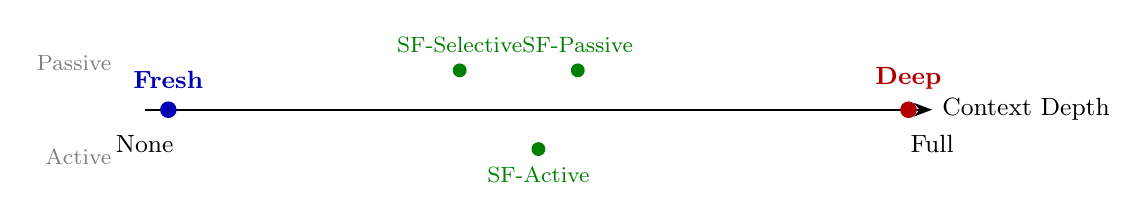
\begin{tikzpicture}[>=Stealth]
  % Axis
  \draw[thick, ->] (0,0) -- (10,0) node[right] {\small Context Depth};
  \node[below, font=\small] at (0, -0.2) {None};
  \node[below, font=\small] at (10, -0.2) {Full};

  % Points
  \fill[blue!70!black] (0.3,0) circle (3pt) node[above=4pt, font=\small\bfseries] {Fresh};
  \fill[red!70!black] (9.7,0) circle (3pt) node[above=4pt, font=\small\bfseries] {Deep};

  % Semi-Fresh variants (in between)
  \fill[green!50!black] (4.0, 0.5) circle (2.5pt) node[above=3pt, font=\footnotesize] {SF-Selective};
  \fill[green!50!black] (5.0,-0.5) circle (2.5pt) node[below=3pt, font=\footnotesize] {SF-Active};
  \fill[green!50!black] (5.5, 0.5) circle (2.5pt) node[above=3pt, font=\footnotesize] {SF-Passive};

  % Delivery mode annotation
  \node[left, font=\footnotesize, text=gray] at (-0.3, 0.6) {Passive};
  \node[left, font=\footnotesize, text=gray] at (-0.3,-0.6) {Active};

\end{tikzpicture}
\caption{Exploration of the Semi-Fresh region in the depth $\times$ delivery space.}
\label{fig:semifresh}
\end{figure}

If Semi-Fresh-Active outperforms both Fresh and Deep, it would suggest that the optimal verification partner is neither ignorant nor entrenched, but \textbf{selectively informed with retrieval autonomy}---a finding with direct implications for how multi-agent systems should manage shared knowledge. If the Active variant outperforms Passive with identical information, it would demonstrate that \textbf{how context is delivered matters independently of what context is delivered}---a novel result absent from the existing MAD literature.

\paragraph{Preliminary results (\S\ref{sec:exp2}).} We implemented and evaluated all three Semi-Fresh variants on the long-context tasks. The results provide initial support for the delivery mode hypothesis:

\begin{itemize}[leftmargin=1.5em]
  \item SF-Active achieved 100\% average recall (tied with Self-Consistency for best), while SF-Passive achieved 89\% (tied with Ploidy). The sole difference is delivery mode.
  \item On the most bias-laden task (DB migration), SF-Active found 5/5 while SF-Passive found only 3/5---with identical compressed information.
  \item SF-Selective (94\%) outperformed SF-Passive (89\%), suggesting negative knowledge is more effective than full summaries for maintaining independence.
\end{itemize}

These observations are from a single run on 3 tasks and require statistical validation, but they shift the question from ``does asymmetry help?'' to ``what is the optimal point in the depth~$\times$~delivery space?''---a quantitatively richer and more practically useful direction.

\subsection{Effort Level as Experimental Variable}
\label{sec:effort}

LLM inference providers increasingly expose \textbf{effort} or \textbf{thinking budget} parameters that control how much computation a model applies to each response. In Claude Code, this manifests as four levels: \texttt{low}, \texttt{medium}, \texttt{high}, and \texttt{max}. This parameter is relevant to context-asymmetric debate for three reasons:

\begin{enumerate}[label=\arabic*., leftmargin=1.5em]
  \item \textbf{Effort--asymmetry interaction}: Higher effort may allow a Deep session to reason through its biases more carefully, potentially reducing the benefit of Fresh perspective. Conversely, higher effort in a Fresh session may compensate for missing context through deeper first-principles reasoning.
  \item \textbf{Effort as confound}: If experiments are conducted at a single effort level, observed effects may not generalize. A method that outperforms at \texttt{high} effort may underperform at \texttt{low} effort if the method's benefit depends on reasoning depth.
  \item \textbf{Cost--quality trade-off}: Lower effort is cheaper. If asymmetric debate at \texttt{medium} effort achieves the same recall as single session at \texttt{max} effort, this has practical cost implications.
\end{enumerate}

We propose a $4 \times k$ factorial design crossing effort levels (\texttt{low}, \texttt{medium}, \texttt{high}, \texttt{max}) with $k$ selected methods (e.g., Single, Ploidy, SF-Active) on the long-context tasks. The experiment runner supports this via \texttt{--effort-sweep}:

\begin{lstlisting}
python experiments/run_experiment.py --long --effort-sweep \
    --methods single,ploidy,sf_active
\end{lstlisting}

Key hypotheses to test:
\begin{itemize}[leftmargin=1.5em]
  \item $H_1$: Effort level has a main effect on recall (higher effort $\to$ higher recall).
  \item $H_2$: There is an effort~$\times$~method interaction---context asymmetry provides greater benefit at lower effort levels, where single sessions are more susceptible to anchoring.
  \item $H_3$: The optimal cost--quality point is asymmetric debate at medium effort, not single session at max effort.
\end{itemize}

Preliminary pilot results on the DB migration task (single run each) suggest effort matters:

\begin{table}[H]
\centering
\caption{Effort level pilot results (DB migration task, single run per cell).}
\label{tab:effort-pilot}
\small
\begin{tabular}{@{}lccc@{}}
\toprule
\textbf{Effort} & \textbf{Single Session} & \textbf{Ploidy} & \textbf{SF-Active} \\
\midrule
Low  & 4F+1P & 4F+1P & ---   \\
High & 3F+2P & 4F+1P & \textbf{5F} \\
Max  & \textbf{5F}    & 4F+1P & ---   \\
\bottomrule
\end{tabular}
\end{table}

\noindent At \texttt{max} effort, Single Session achieves 5/5 (matching SF-Active at \texttt{high}), while Ploidy remains at 4F+1P across all effort levels. This is consistent with $H_2$: context asymmetry provides greater benefit at moderate effort, while at maximum effort a single session may overcome anchoring through deeper reasoning alone. These are single-run observations subject to stochastic variance.

\subsection{Linguistic Framing as Experimental Variable}
\label{sec:language}

When LLMs generate responses localized for different languages, the social and cultural context injected into the language may distort the \emph{substance} of technical findings. This is a form of information loss distinct from context anchoring but potentially compounding it.

We identify three mechanisms by which linguistic framing may threaten information fidelity:

\begin{enumerate}[label=\arabic*., leftmargin=1.5em]
  \item \textbf{Euphemization}: Languages with strong politeness norms (Korean, Japanese) may soften critical findings. ``This code has a critical SQL injection vulnerability'' becomes ``There may be room for improvement in input handling''---the severity signal is lost.
  \item \textbf{Hierarchical suppression}: In languages with grammatical honorifics (Korean's \emph{jondaenmal}/\emph{banmal}, Japanese's \emph{keigo}), challenges to established positions may be linguistically weakened. A Fresh session challenging a Deep session's position may unconsciously soften its critique when generating in Korean, reducing the effectiveness of the adversarial signal.
  \item \textbf{Technical term dilution}: When technical terms are translated rather than preserved (e.g., ``race condition'' $\to$ ``경쟁 상태''), the precision of the finding may decrease, and the judge may have difficulty matching translated findings to English-language ground truth.
\end{enumerate}

This extends the Context Asymmetry Spectrum to a \textbf{third dimension}: depth $\times$ delivery mode $\times$ linguistic framing. We propose a language sweep experiment:

\begin{lstlisting}
python experiments/run_experiment.py --long --lang-sweep \
    --methods single,ploidy --langs en,ko,ja,zh
\end{lstlisting}

Key hypotheses:
\begin{itemize}[leftmargin=1.5em]
  \item $H_1$: Localized responses achieve lower recall on English-language ground truth due to euphemization and term dilution.
  \item $H_2$: The recall gap between languages is larger for Fresh sessions (which lack context to anchor technical vocabulary) than Deep sessions.
  \item $H_3$: Context asymmetry may \emph{partially compensate} for localization loss---if the Fresh session in language $L$ misses an issue due to euphemization, the Deep session (with stronger technical framing from project context) may catch it during the challenge phase.
\end{itemize}

Preliminary pilot results on the DB migration task (Korean vs.\ English, \texttt{high} effort, single run each):

\begin{table}[H]
\centering
\caption{Language pilot results (DB migration task, single run per cell).}
\label{tab:lang-pilot}
\small
\begin{tabular}{@{}lccc@{}}
\toprule
\textbf{Language} & \textbf{Single Session} & \textbf{Ploidy} & \textbf{SF-Active} \\
\midrule
English & 3F+2P & 4F+1P & \textbf{5F} \\
Korean  & \textbf{5F}    & 4F+1P & 2F+3P \\
\bottomrule
\end{tabular}
\end{table}

\noindent The most striking observation is SF-Active's recall drop in Korean: from 5/5 (\textsc{found}) in English to 2/5 \textsc{found} + 3 \textsc{partial} in Korean---a 30 percentage point decline. This is consistent with $H_1$ (euphemization): the Korean ``independent analysis then consult summary'' workflow may produce softer language that the English-language judge scores as \textsc{partial} rather than \textsc{found}. Conversely, Single Session's Korean performance (5F) exceeds its English performance (3F+2P), suggesting that full project context may provide technical vocabulary anchoring that resists euphemization. These are single-run observations requiring validation, but they motivate systematic cross-linguistic evaluation.

\subsection{Limitations}
\label{sec:limitations}

This pilot study has significant limitations that bound the strength of all claims:

\begin{itemize}[leftmargin=1.5em]
  \item \textbf{Statistical power}: 7+3 tasks, single run per method-task pair (re-run on Exp~2 only). Observed method differences (F1 $\Delta \approx 0.03$) are smaller than within-method variance (F1 $\Delta \approx 0.10$). No statistical tests are reported because the sample size and run count cannot support them. Minimum requirement for validated claims: 30+ tasks, 5+ runs, paired statistical tests (Wilcoxon signed-rank or bootstrap CI).
  \item \textbf{Author-defined ground truth}: All ground-truth issues were defined by the authors without independent expert validation. Bonus findings identified by the judge suggest the ground truth is incomplete. Future work should use independently validated benchmarks or multiple expert annotators with inter-rater agreement metrics.
  \item \textbf{Single model family}: All experiments use Claude Opus 4.6 for generation. Observed effects may be Claude-specific---different model families (GPT-4o, Gemini 2.5) may exhibit different anchoring dynamics, context sensitivity, or debate behavior. Cross-model replication with at least two additional model families is necessary before generalizability claims.
  \item \textbf{Same-model judge}: Claude Opus 4.6 generates outputs and evaluates them. Systematic bias is possible (e.g., preference for structured multi-phase outputs, or conversely, penalizing verbose responses). Cross-model judges (GPT-4, Gemini) and a human evaluation subset with Cohen's kappa are needed.
  \item \textbf{Circular task design risk}: Long-context tasks were designed with anchoring biases whose detection is facilitated by context absence. A session without context is expected to be less biased by definition. Stronger validation requires externally-sourced tasks (e.g., real-world architecture decisions from open-source projects) where the relationship between context and bias is not author-designed.
  \item \textbf{Token cost}: Ploidy uses approximately 5$\times$ the tokens of Single Session. Self-Consistency (5-vote) was included as a budget-equivalent baseline and achieves the same 100\% recall as SF-Active on long-context tasks. The practical advantage of structured debate over Self-Consistency is the typed audit trail and convergence analysis, not recall improvement---a distinction that may or may not justify the added protocol complexity.
  \item \textbf{CLI simulation vs.\ MCP server}: Experiments use \texttt{claude --print} CLI rather than the Ploidy MCP server. While this provides cleaner session isolation, the convergence engine's rule-based classification (in the server) is not exercised in the experiments.
  \item \textbf{Metric design}: The current F1 formulation penalizes valid bonus findings as false positives. This systematically disadvantages more thorough methods and should be revised in future work.
  \item \textbf{Single effort level}: All experiments use the default \texttt{high} effort setting. Results may differ at other effort levels, and effort--method interactions are unmeasured (\S\ref{sec:effort}).
  \item \textbf{English-only evaluation}: All experiments and ground truth are in English. Localized responses in other languages may exhibit different anchoring dynamics and information loss patterns (\S\ref{sec:language}).
\end{itemize}

\subsection{Broader Implications}
\label{sec:implications}

The stochastic prior lock-in problem is not unique to LLMs---it mirrors well-documented phenomena in human organizations where accumulated context simultaneously enables domain mastery and prevents paradigm revision~\citep{kuhn1962structure, azoulay2019funeral}. A companion paper formalizes this structural isomorphism between LLM context windows and human generational dynamics, including the connection to model collapse~\citep{shumailov2024collapse} as the failure mode when generational context asymmetry is absent.

For multi-agent system design, our preliminary results suggest a practical principle: \textbf{context diversity may be more valuable than agent count}. Combined with Choi et al.'s martingale result~\citep{choi2025debate} (scaling homogeneous agents cannot improve expected correctness) and Boca et al.'s finding~\citep{boca2025emergent} that LLM populations spontaneously develop collective biases, this motivates architectures that deliberately maintain sessions with different context depths rather than scaling identical agents.

% ============================================================
\section{Conclusion and Future Work}
\label{sec:conclusion}
% ============================================================

We presented Ploidy, a protocol for structured debate between same-model sessions with intentional context asymmetry, and introduced the Context Asymmetry Spectrum---a 2D framework varying context depth and delivery mode. Three pilot experiments across 10 tasks and 9 methods reveal:

\begin{enumerate}[label=\arabic*., leftmargin=1.5em]
  \item \textbf{Context asymmetry is a targeted intervention}, not a universal improvement. On short-context tasks (Exp~1, 7 tasks), all 9 methods achieve near-identical recall. The delivery mode effect disappears entirely.
  \item \textbf{On long-context tasks with anchoring bias} (Exp~2, 3 tasks), Semi-Fresh-Active and Self-Consistency achieve 100\% average recall, outperforming Single Session (81\%) and original Ploidy (89\%).
  \item \textbf{Information position is the dominant factor in context delivery.} Factorial ablation reveals that placing a compressed summary at the top vs.\ bottom of the prompt accounts for +11pp recall (89\% $\to$ 100\%), while an ``independent-first'' instruction adds only +5pp when the summary is at the top and +0pp when at the bottom. This primacy anchoring effect---where information encountered first disproportionately shapes subsequent reasoning---is consistent with established cognitive science findings~\citep{epley2006anchoring} and has direct implications for prompt engineering in multi-agent systems.
\end{enumerate}

These results shift the question from ``does asymmetry help?'' to ``what is the optimal point in the depth~$\times$~delivery space?''---a quantitatively richer direction with direct implications for multi-agent system design.

\paragraph{Future work priorities:}
\begin{enumerate}[label=\arabic*., leftmargin=1.5em]
  \item \textbf{Effort level sweep}: Execute the $4 \times k$ factorial experiment (\S\ref{sec:effort}) to measure effort--asymmetry interaction and identify cost-optimal configurations
  \item \textbf{N-ary session topology}: Extend beyond binary (Deep/Fresh) to three-party debates with intermediate context levels (Deep + Semi-Fresh + Fresh), testing whether partial context sessions produce novel insights absent from both extremes
  \item \textbf{LLM-enhanced convergence validation}: Evaluate whether the meta-analyst's root cause attribution (context anchoring vs.\ missing constraints vs.\ genuine trade-off) aligns with human expert judgment
  \item \textbf{Statistical validation}: 30+ tasks, 5+ runs per method, paired statistical tests (Wilcoxon signed-rank, bootstrap CI)
  \item \textbf{Context-length gradient}: systematic evaluation at 100, 500, 1K, 5K, 10K tokens to identify the entrenchment threshold
  \item \textbf{Cross-model evaluation}: weaker models (where single-session recall is lower) and cross-model judges
  \item \textbf{External task sets}: real-world architecture decisions from open-source projects to address circular task design concerns
  \item \textbf{Multi-round protocol}: extending the single-round \textsc{challenge} phase to test whether AceMAD's submartingale conditions can be satisfied
  \item \textbf{Production validation}: Compare MCP server debate (\texttt{debate\_auto}) outcomes with CLI simulation to validate that the server protocol produces equivalent results
  \item \textbf{Cross-linguistic evaluation}: Measure information loss from linguistic framing across languages (English, Korean, Japanese, Chinese) and test whether context asymmetry compensates for localization-induced euphemization (\S\ref{sec:language})
\end{enumerate}

We release Ploidy as an open-source MCP server at \url{https://github.com/heznpc/ploidy}.

% ============================================================
\section*{Acknowledgments}
% ============================================================

This paper was written with the assistance of Claude Code (Anthropic, Claude Opus 4.6). The experimental framework, literature search, and draft editing were conducted through interactive sessions with the tool. All research decisions, hypotheses, and interpretations are the authors' own.

% ============================================================
% References
% ============================================================
% These references appear in the original reference list but are not cited in the body.
% \nocite ensures they are included in the bibliography for completeness.
\nocite{debate2026deliberation}
\bibliography{references}

\end{document}
